\documentclass{standalone}
\usepackage{tikz}
\usetikzlibrary{patterns, positioning}

\begin{document}
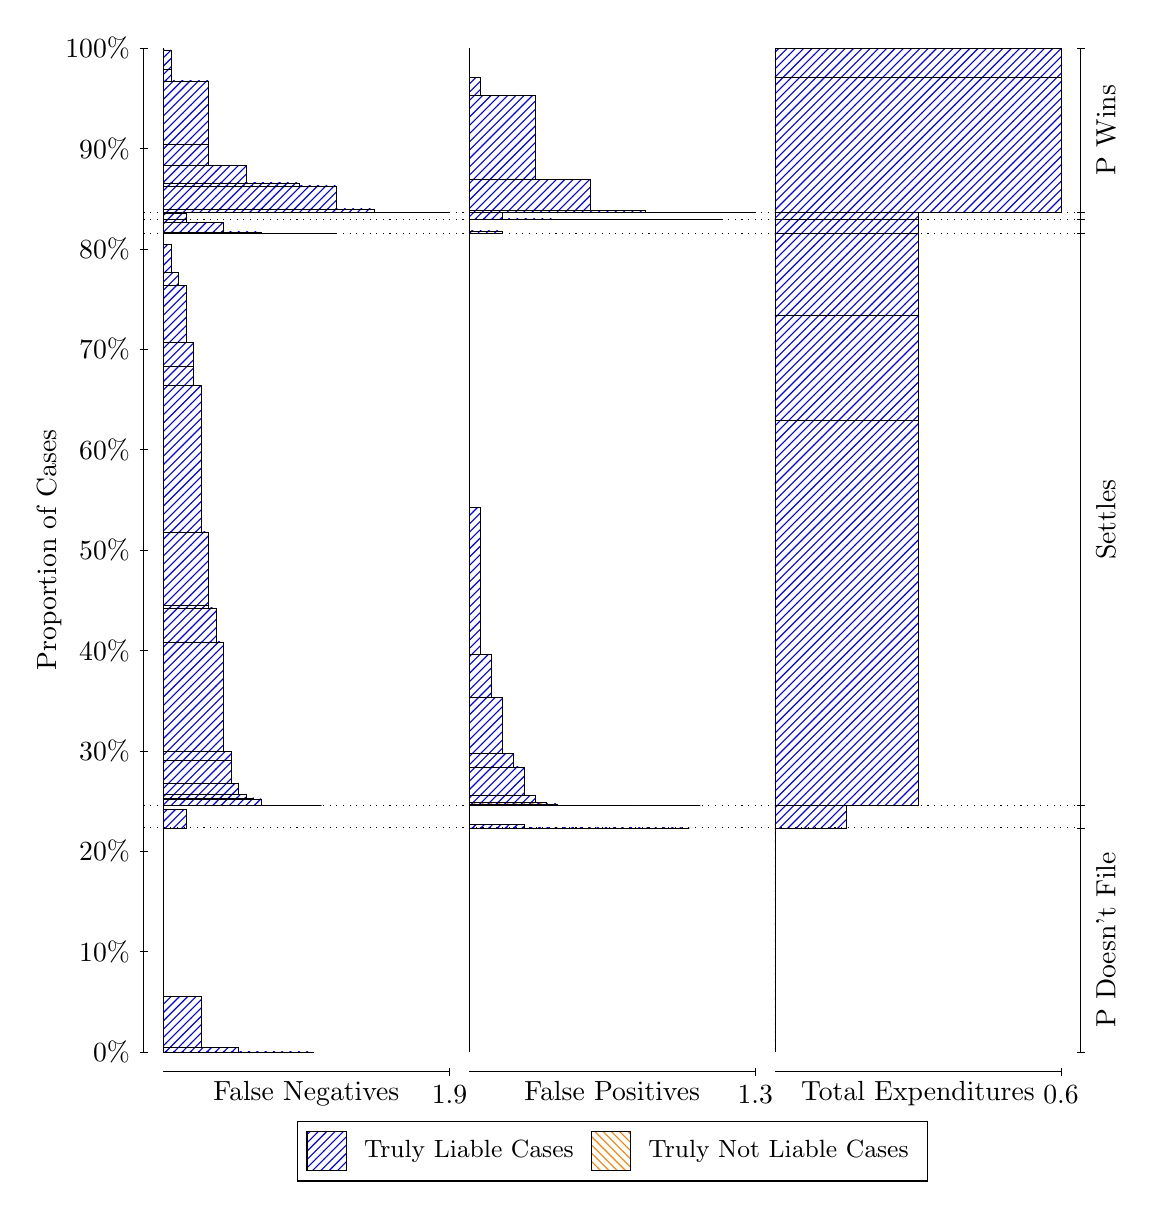
\begin{tikzpicture}
\draw[black, very thin] (1.5,1.75) -- (1.5,14.5);
\node[rotate=90, anchor=center] at (0.3, 8.125) {Proportion of Cases};
\draw[black, very thin] (1.45,1.75) -- (1.55,1.75);
\node[anchor=east] at (1.45, 1.75) {0\%};
\draw[black, very thin] (1.45,3.025) -- (1.55,3.025);
\node[anchor=east] at (1.45, 3.025) {10\%};
\draw[black, very thin] (1.45,4.3) -- (1.55,4.3);
\node[anchor=east] at (1.45, 4.3) {20\%};
\draw[black, very thin] (1.45,5.575) -- (1.55,5.575);
\node[anchor=east] at (1.45, 5.575) {30\%};
\draw[black, very thin] (1.45,6.85) -- (1.55,6.85);
\node[anchor=east] at (1.45, 6.85) {40\%};
\draw[black, very thin] (1.45,8.125) -- (1.55,8.125);
\node[anchor=east] at (1.45, 8.125) {50\%};
\draw[black, very thin] (1.45,9.4) -- (1.55,9.4);
\node[anchor=east] at (1.45, 9.4) {60\%};
\draw[black, very thin] (1.45,10.675) -- (1.55,10.675);
\node[anchor=east] at (1.45, 10.675) {70\%};
\draw[black, very thin] (1.45,11.95) -- (1.55,11.95);
\node[anchor=east] at (1.45, 11.95) {80\%};
\draw[black, very thin] (1.45,13.225) -- (1.55,13.225);
\node[anchor=east] at (1.45, 13.225) {90\%};
\draw[black, very thin] (1.45,14.5) -- (1.55,14.5);
\node[anchor=east] at (1.45, 14.5) {100\%};

\draw[black, very thin] (13.4,1.75) -- (13.4,14.5);
\draw[black, very thin] (13.35,1.75) -- (13.45,1.75);
\node[anchor=west] at (13.35, 1.75) {};
\draw[black, very thin] (13.35,4.5952) -- (13.45,4.5952);
\node[anchor=west] at (13.35, 4.5952) {};
\draw[black, very thin] (13.35,4.8772) -- (13.45,4.8772);
\node[anchor=west] at (13.35, 4.8772) {};
\draw[black, very thin] (13.35,12.143) -- (13.45,12.143);
\node[anchor=west] at (13.35, 12.143) {};
\draw[black, very thin] (13.35,12.32) -- (13.45,12.32);
\node[anchor=west] at (13.35, 12.32) {};
\draw[black, very thin] (13.35,12.413) -- (13.45,12.413);
\node[anchor=west] at (13.35, 12.413) {};
\draw[black, very thin] (13.35,14.5) -- (13.45,14.5);
\node[anchor=west] at (13.35, 14.5) {};

\draw[black, very thin, pattern color=blue, pattern=north east lines] (1.75,1.75) rectangle (3.6623,1.75);
\draw[black, very thin, pattern color=blue, pattern=north east lines] (1.75,1.75) rectangle (3.1842,1.7505);
\draw[black, very thin, pattern color=blue, pattern=north east lines] (1.75,1.7505) rectangle (2.7061,1.8106);
\draw[black, very thin, pattern color=blue, pattern=north east lines] (1.75,1.8106) rectangle (2.2281,2.4587);
\draw[black, very thin, pattern color=orange, pattern=north west lines] (1.75,2.4587) rectangle (1.75,2.4587);
\draw[black, very thin, pattern color=blue, pattern=north east lines] (1.75,2.4587) rectangle (1.75,4.5952);
\draw[black, very thin, pattern color=blue, pattern=north east lines] (1.75,4.5952) rectangle (2.0368,4.831);
\draw[black, very thin, pattern color=orange, pattern=north west lines] (1.75,4.831) rectangle (1.75,4.831);
\draw[black, very thin, pattern color=blue, pattern=north east lines] (1.75,4.831) rectangle (1.75,4.8772);
\draw[black, very thin, pattern color=blue, pattern=north east lines] (1.75,4.8772) rectangle (3.7579,4.8772);
\draw[black, very thin, pattern color=blue, pattern=north east lines] (1.75,4.8772) rectangle (3.5667,4.8772);
\draw[black, very thin, pattern color=blue, pattern=north east lines] (1.75,4.8772) rectangle (3.3754,4.8772);
\draw[black, very thin, pattern color=blue, pattern=north east lines] (1.75,4.8772) rectangle (3.2798,4.8772);
\draw[black, very thin, pattern color=blue, pattern=north east lines] (1.75,4.8772) rectangle (3.1842,4.8776);
\draw[black, very thin, pattern color=blue, pattern=north east lines] (1.75,4.8776) rectangle (3.0886,4.8778);
\draw[black, very thin, pattern color=blue, pattern=north east lines] (1.75,4.8778) rectangle (2.993,4.9633);
\draw[black, very thin, pattern color=blue, pattern=north east lines] (1.75,4.9633) rectangle (2.8974,4.9782);
\draw[black, very thin, pattern color=blue, pattern=north east lines] (1.75,4.9782) rectangle (2.8018,5.0221);
\draw[black, very thin, pattern color=blue, pattern=north east lines] (1.75,5.0221) rectangle (2.7061,5.1598);
\draw[black, very thin, pattern color=blue, pattern=north east lines] (1.75,5.1598) rectangle (2.6105,5.4569);
\draw[black, very thin, pattern color=blue, pattern=north east lines] (1.75,5.4569) rectangle (2.6105,5.563);
\draw[black, very thin, pattern color=blue, pattern=north east lines] (1.75,5.563) rectangle (2.5149,6.9586);
\draw[black, very thin, pattern color=blue, pattern=north east lines] (1.75,6.9586) rectangle (2.4193,7.3905);
\draw[black, very thin, pattern color=blue, pattern=north east lines] (1.75,7.3905) rectangle (2.3237,7.4173);
\draw[black, very thin, pattern color=blue, pattern=north east lines] (1.75,7.4173) rectangle (2.3237,8.3552);
\draw[black, very thin, pattern color=blue, pattern=north east lines] (1.75,8.3552) rectangle (2.2281,10.218);
\draw[black, very thin, pattern color=blue, pattern=north east lines] (1.75,10.218) rectangle (2.1325,10.458);
\draw[black, very thin, pattern color=blue, pattern=north east lines] (1.75,10.458) rectangle (2.1325,10.762);
\draw[black, very thin, pattern color=blue, pattern=north east lines] (1.75,10.762) rectangle (2.0368,11.483);
\draw[black, very thin, pattern color=blue, pattern=north east lines] (1.75,11.483) rectangle (1.9412,11.651);
\draw[black, very thin, pattern color=blue, pattern=north east lines] (1.75,11.651) rectangle (1.9412,11.651);
\draw[black, very thin, pattern color=blue, pattern=north east lines] (1.75,11.651) rectangle (1.8456,11.652);
\draw[black, very thin, pattern color=blue, pattern=north east lines] (1.75,11.652) rectangle (1.8456,12.008);
\draw[black, very thin, pattern color=blue, pattern=north east lines] (1.75,12.008) rectangle (1.75,12.008);
\draw[black, very thin, pattern color=orange, pattern=north west lines] (1.75,12.008) rectangle (1.75,12.008);
\draw[black, very thin, pattern color=blue, pattern=north east lines] (1.75,12.008) rectangle (1.75,12.143);
\draw[black, very thin, pattern color=blue, pattern=north east lines] (1.75,12.143) rectangle (3.9491,12.143);
\draw[black, very thin, pattern color=blue, pattern=north east lines] (1.75,12.143) rectangle (3.4711,12.143);
\draw[black, very thin, pattern color=blue, pattern=north east lines] (1.75,12.143) rectangle (2.993,12.164);
\draw[black, very thin, pattern color=blue, pattern=north east lines] (1.75,12.164) rectangle (2.5149,12.284);
\draw[black, very thin, pattern color=blue, pattern=north east lines] (1.75,12.284) rectangle (2.0368,12.32);
\draw[black, very thin, pattern color=orange, pattern=north west lines] (1.75,12.32) rectangle (1.75,12.32);
\draw[black, very thin, pattern color=blue, pattern=north east lines] (1.75,12.32) rectangle (2.0368,12.403);
\draw[black, very thin, pattern color=orange, pattern=north west lines] (1.75,12.403) rectangle (1.75,12.403);
\draw[black, very thin, pattern color=blue, pattern=north east lines] (1.75,12.403) rectangle (1.75,12.413);
\draw[black, very thin, pattern color=blue, pattern=north east lines] (1.75,12.413) rectangle (5.3833,12.413);
\draw[black, very thin, pattern color=blue, pattern=north east lines] (1.75,12.413) rectangle (4.9053,12.414);
\draw[black, very thin, pattern color=blue, pattern=north east lines] (1.75,12.414) rectangle (4.4272,12.456);
\draw[black, very thin, pattern color=blue, pattern=north east lines] (1.75,12.456) rectangle (3.9491,12.748);
\draw[black, very thin, pattern color=blue, pattern=north east lines] (1.75,12.748) rectangle (3.7579,12.748);
\draw[black, very thin, pattern color=blue, pattern=north east lines] (1.75,12.748) rectangle (3.4711,12.787);
\draw[black, very thin, pattern color=blue, pattern=north east lines] (1.75,12.787) rectangle (3.2798,12.787);
\draw[black, very thin, pattern color=blue, pattern=north east lines] (1.75,12.787) rectangle (2.993,12.787);
\draw[black, very thin, pattern color=blue, pattern=north east lines] (1.75,12.787) rectangle (2.8018,13.01);
\draw[black, very thin, pattern color=blue, pattern=north east lines] (1.75,13.01) rectangle (2.5149,13.01);
\draw[black, very thin, pattern color=blue, pattern=north east lines] (1.75,13.01) rectangle (2.3237,13.274);
\draw[black, very thin, pattern color=blue, pattern=north east lines] (1.75,13.274) rectangle (2.3237,14.082);
\draw[black, very thin, pattern color=blue, pattern=north east lines] (1.75,14.082) rectangle (1.8456,14.224);
\draw[black, very thin, pattern color=blue, pattern=north east lines] (1.75,14.224) rectangle (1.8456,14.475);
\draw[black, very thin, pattern color=orange, pattern=north west lines] (1.75,14.475) rectangle (1.75,14.475);
\draw[black, very thin, pattern color=blue, pattern=north east lines] (1.75,14.475) rectangle (1.75,14.5);
\draw[black, very thin, pattern color=orange, pattern=north west lines] (5.6333,1.75) rectangle (5.6333,1.75);
\draw[black, very thin, pattern color=blue, pattern=north east lines] (5.6333,1.75) rectangle (5.6333,4.5952);
\draw[black, very thin, pattern color=orange, pattern=north west lines] (5.6333,4.5952) rectangle (8.4282,4.5952);
\draw[black, very thin, pattern color=blue, pattern=north east lines] (5.6333,4.5952) rectangle (8.4282,4.5952);
\draw[black, very thin, pattern color=blue, pattern=north east lines] (5.6333,4.5952) rectangle (7.7295,4.5952);
\draw[black, very thin, pattern color=blue, pattern=north east lines] (5.6333,4.5952) rectangle (7.0308,4.5956);
\draw[black, very thin, pattern color=blue, pattern=north east lines] (5.6333,4.5956) rectangle (6.3321,4.6414);
\draw[black, very thin, pattern color=blue, pattern=north east lines] (5.6333,4.6414) rectangle (5.6333,4.8772);
\draw[black, very thin, pattern color=orange, pattern=north west lines] (5.6333,4.8772) rectangle (8.5679,4.8772);
\draw[black, very thin, pattern color=blue, pattern=north east lines] (5.6333,4.8772) rectangle (8.5679,4.8772);
\draw[black, very thin, pattern color=orange, pattern=north west lines] (5.6333,4.8772) rectangle (8.2885,4.8772);
\draw[black, very thin, pattern color=blue, pattern=north east lines] (5.6333,4.8772) rectangle (8.2885,4.8772);
\draw[black, very thin, pattern color=orange, pattern=north west lines] (5.6333,4.8772) rectangle (8.009,4.8772);
\draw[black, very thin, pattern color=blue, pattern=north east lines] (5.6333,4.8772) rectangle (8.009,4.8772);
\draw[black, very thin, pattern color=blue, pattern=north east lines] (5.6333,4.8772) rectangle (7.8692,4.8772);
\draw[black, very thin, pattern color=orange, pattern=north west lines] (5.6333,4.8772) rectangle (7.7295,4.8772);
\draw[black, very thin, pattern color=blue, pattern=north east lines] (5.6333,4.8772) rectangle (7.7295,4.8772);
\draw[black, very thin, pattern color=blue, pattern=north east lines] (5.6333,4.8772) rectangle (7.5897,4.8772);
\draw[black, very thin, pattern color=orange, pattern=north west lines] (5.6333,4.8772) rectangle (7.45,4.8772);
\draw[black, very thin, pattern color=blue, pattern=north east lines] (5.6333,4.8772) rectangle (7.45,4.8772);
\draw[black, very thin, pattern color=blue, pattern=north east lines] (5.6333,4.8772) rectangle (7.3103,4.8772);
\draw[black, very thin, pattern color=orange, pattern=north west lines] (5.6333,4.8772) rectangle (7.1705,4.8772);
\draw[black, very thin, pattern color=blue, pattern=north east lines] (5.6333,4.8772) rectangle (7.1705,4.8773);
\draw[black, very thin, pattern color=orange, pattern=north west lines] (5.6333,4.8773) rectangle (7.1705,4.8773);
\draw[black, very thin, pattern color=blue, pattern=north east lines] (5.6333,4.8773) rectangle (7.1705,4.8773);
\draw[black, very thin, pattern color=blue, pattern=north east lines] (5.6333,4.8773) rectangle (7.0308,4.8773);
\draw[black, very thin, pattern color=blue, pattern=north east lines] (5.6333,4.8773) rectangle (6.891,4.8773);
\draw[black, very thin, pattern color=orange, pattern=north west lines] (5.6333,4.8773) rectangle (6.891,4.8773);
\draw[black, very thin, pattern color=blue, pattern=north east lines] (5.6333,4.8773) rectangle (6.891,4.878);
\draw[black, very thin, pattern color=blue, pattern=north east lines] (5.6333,4.878) rectangle (6.7513,4.9011);
\draw[black, very thin, pattern color=orange, pattern=north west lines] (5.6333,4.9011) rectangle (6.6115,4.9011);
\draw[black, very thin, pattern color=blue, pattern=north east lines] (5.6333,4.9011) rectangle (6.6115,4.9185);
\draw[black, very thin, pattern color=blue, pattern=north east lines] (5.6333,4.9185) rectangle (6.4718,5.012);
\draw[black, very thin, pattern color=blue, pattern=north east lines] (5.6333,5.012) rectangle (6.4718,5.012);
\draw[black, very thin, pattern color=orange, pattern=north west lines] (5.6333,5.012) rectangle (6.3321,5.012);
\draw[black, very thin, pattern color=blue, pattern=north east lines] (5.6333,5.012) rectangle (6.3321,5.3696);
\draw[black, very thin, pattern color=blue, pattern=north east lines] (5.6333,5.3696) rectangle (6.1923,5.3696);
\draw[black, very thin, pattern color=blue, pattern=north east lines] (5.6333,5.3696) rectangle (6.1923,5.5376);
\draw[black, very thin, pattern color=blue, pattern=north east lines] (5.6333,5.5376) rectangle (6.0526,6.2581);
\draw[black, very thin, pattern color=blue, pattern=north east lines] (5.6333,6.2581) rectangle (5.9128,6.8018);
\draw[black, very thin, pattern color=blue, pattern=north east lines] (5.6333,6.8018) rectangle (5.7731,8.6651);
\draw[black, very thin, pattern color=blue, pattern=north east lines] (5.6333,8.6651) rectangle (5.7731,8.6651);
\draw[black, very thin, pattern color=blue, pattern=north east lines] (5.6333,8.6651) rectangle (5.6333,12.143);
\draw[black, very thin, pattern color=orange, pattern=north west lines] (5.6333,12.143) rectangle (6.0526,12.143);
\draw[black, very thin, pattern color=blue, pattern=north east lines] (5.6333,12.143) rectangle (6.0526,12.179);
\draw[black, very thin, pattern color=blue, pattern=north east lines] (5.6333,12.179) rectangle (5.6333,12.32);
\draw[black, very thin, pattern color=orange, pattern=north west lines] (5.6333,12.32) rectangle (8.8474,12.32);
\draw[black, very thin, pattern color=blue, pattern=north east lines] (5.6333,12.32) rectangle (8.8474,12.32);
\draw[black, very thin, pattern color=blue, pattern=north east lines] (5.6333,12.32) rectangle (8.1487,12.32);
\draw[black, very thin, pattern color=blue, pattern=north east lines] (5.6333,12.32) rectangle (7.45,12.321);
\draw[black, very thin, pattern color=blue, pattern=north east lines] (5.6333,12.321) rectangle (6.7513,12.331);
\draw[black, very thin, pattern color=blue, pattern=north east lines] (5.6333,12.331) rectangle (6.0526,12.413);
\draw[black, very thin, pattern color=orange, pattern=north west lines] (5.6333,12.413) rectangle (9.2667,12.413);
\draw[black, very thin, pattern color=blue, pattern=north east lines] (5.6333,12.413) rectangle (9.2667,12.413);
\draw[black, very thin, pattern color=orange, pattern=north west lines] (5.6333,12.413) rectangle (8.5679,12.413);
\draw[black, very thin, pattern color=blue, pattern=north east lines] (5.6333,12.413) rectangle (8.5679,12.413);
\draw[black, very thin, pattern color=orange, pattern=north west lines] (5.6333,12.413) rectangle (7.8692,12.413);
\draw[black, very thin, pattern color=blue, pattern=north east lines] (5.6333,12.413) rectangle (7.8692,12.438);
\draw[black, very thin, pattern color=orange, pattern=north west lines] (5.6333,12.438) rectangle (7.1705,12.438);
\draw[black, very thin, pattern color=blue, pattern=north east lines] (5.6333,12.438) rectangle (7.1705,12.831);
\draw[black, very thin, pattern color=blue, pattern=north east lines] (5.6333,12.831) rectangle (6.4718,13.903);
\draw[black, very thin, pattern color=orange, pattern=north west lines] (5.6333,13.903) rectangle (6.1923,13.903);
\draw[black, very thin, pattern color=blue, pattern=north east lines] (5.6333,13.903) rectangle (6.1923,13.903);
\draw[black, very thin, pattern color=blue, pattern=north east lines] (5.6333,13.903) rectangle (5.7731,14.126);
\draw[black, very thin, pattern color=orange, pattern=north west lines] (5.6333,14.126) rectangle (5.6333,14.126);
\draw[black, very thin, pattern color=blue, pattern=north east lines] (5.6333,14.126) rectangle (5.6333,14.5);
\draw[black, very thin, pattern color=orange, pattern=north west lines] (9.5167,1.75) rectangle (9.5167,1.75);
\draw[black, very thin, pattern color=blue, pattern=north east lines] (9.5167,1.75) rectangle (9.5167,4.5952);
\draw[black, very thin, pattern color=orange, pattern=north west lines] (9.5167,4.5952) rectangle (10.425,4.5952);
\draw[black, very thin, pattern color=blue, pattern=north east lines] (9.5167,4.5952) rectangle (10.425,4.8772);
\draw[black, very thin, pattern color=orange, pattern=north west lines] (9.5167,4.8772) rectangle (11.333,4.8772);
\draw[black, very thin, pattern color=blue, pattern=north east lines] (9.5167,4.8772) rectangle (11.333,9.7678);
\draw[black, very thin, pattern color=orange, pattern=north west lines] (9.5167,9.7678) rectangle (11.333,9.7678);
\draw[black, very thin, pattern color=blue, pattern=north east lines] (9.5167,9.7678) rectangle (11.333,11.101);
\draw[black, very thin, pattern color=orange, pattern=north west lines] (9.5167,11.101) rectangle (11.333,11.101);
\draw[black, very thin, pattern color=blue, pattern=north east lines] (9.5167,11.101) rectangle (11.333,12.143);
\draw[black, very thin, pattern color=orange, pattern=north west lines] (9.5167,12.143) rectangle (11.333,12.143);
\draw[black, very thin, pattern color=blue, pattern=north east lines] (9.5167,12.143) rectangle (11.333,12.32);
\draw[black, very thin, pattern color=orange, pattern=north west lines] (9.5167,12.32) rectangle (11.333,12.32);
\draw[black, very thin, pattern color=blue, pattern=north east lines] (9.5167,12.32) rectangle (11.333,12.413);
\draw[black, very thin, pattern color=orange, pattern=north west lines] (9.5167,12.413) rectangle (13.15,12.413);
\draw[black, very thin, pattern color=blue, pattern=north east lines] (9.5167,12.413) rectangle (13.15,14.126);
\draw[black, very thin, pattern color=orange, pattern=north west lines] (9.5167,14.126) rectangle (13.15,14.126);
\draw[black, very thin, pattern color=blue, pattern=north east lines] (9.5167,14.126) rectangle (13.15,14.5);
\draw[black, dotted] (1.5,4.5952) -- (13.4,4.5952);
\draw[black, dotted] (1.5,4.8772) -- (13.4,4.8772);
\draw[black, dotted] (1.5,12.143) -- (13.4,12.143);
\draw[black, dotted] (1.5,12.32) -- (13.4,12.32);
\draw[black, dotted] (1.5,12.413) -- (13.4,12.413);
\draw[black, very thin] (1.75,1.5) -- (5.3833,1.5);
\node[anchor=north] at (3.5667, 1.5) {False Negatives};
\draw[black, very thin] (5.3833,1.45) -- (5.3833,1.55);
\node[anchor=north] at (5.3833, 1.45) {1.9};

\draw[black, very thin] (5.6333,1.5) -- (9.2667,1.5);
\node[anchor=north] at (7.45, 1.5) {False Positives};
\draw[black, very thin] (9.2667,1.45) -- (9.2667,1.55);
\node[anchor=north] at (9.2667, 1.45) {1.3};

\draw[black, very thin] (9.5167,1.5) -- (13.15,1.5);
\node[anchor=north] at (11.333, 1.5) {Total Expenditures};
\draw[black, very thin] (13.15,1.45) -- (13.15,1.55);
\node[anchor=north] at (13.15, 1.45) {0.6};

\node[black, centered, rotate=90] at (13.72, 3.1726) {P Doesn't File};

\node[black, centered, rotate=90] at (13.72, 8.5102) {Settles};


\node[black, centered, rotate=90] at (13.72, 13.457) {P Wins};

\draw (7.449999999999999,1.5) node[draw=none] (baseCoordinate) {};
\begin{scope}[align=center]
        \matrix[scale=0.5, draw=black, below=0.5cm of baseCoordinate, nodes={draw}, column sep=0.1cm]{
            \node[rectangle, draw, minimum width=0.5cm, minimum height=0.5cm, pattern=north east lines, pattern color=blue] {}; &
            \node[draw=none, font=\small] (B) {Truly Liable Cases}; &
            \node[rectangle, draw, minimum width=0.5cm, minimum height=0.5cm, pattern=north west lines, pattern color=orange] {}; &
            \node[draw=none, font=\small] (B) {Truly Not Liable Cases}; \\
            };
\end{scope}

\end{tikzpicture}
\end{document}